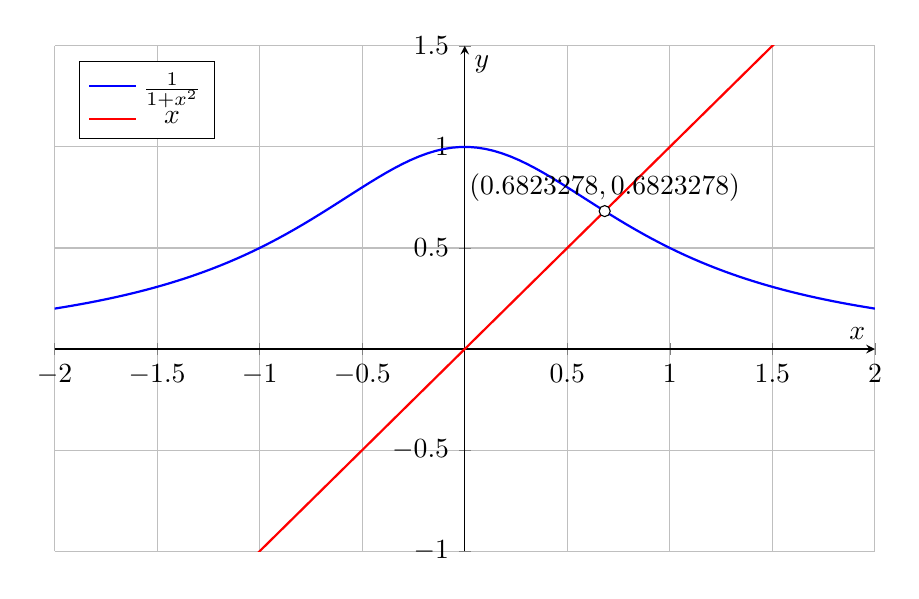
\begin{tikzpicture}
    \begin{axis}[
        axis lines = middle,
        grid = both,
        xlabel = {$x$},
        ylabel = {$y$},
        xmin = -2, xmax = 2,
        ymin = -1.0, ymax = 1.5,
        legend pos = north west,
        width = 12cm, height = 8cm,
        samples = 100,
        domain = -2:2,
    ]
    
    % Plot of 1/(1+x^2)
    \addplot[
        blue,
        thick,
    ]
    {1/(1 + x^2)};
    \addlegendentry{$\frac{1}{1 + x^2}$}

    % Plot of x
    \addplot[
        red,
        thick,
    ]
    {x};
    \addlegendentry{$x$}
    
    % Intersection point
    \addplot[
        mark=*,
        mark options={fill=white},
        only marks,
        nodes near coords,
        point meta=explicit symbolic
    ] coordinates {
        (0.6823278,0.6823278) [$(0.6823278, 0.6823278)$]
    };
    
    \end{axis}
\end{tikzpicture}